\documentclass[12pt,a4paper]{article}

\usepackage[a4paper,margin=1in]{geometry}
\usepackage{graphicx}
\usepackage{hyperref}
\usepackage{longtable}
\usepackage{listings}

\hypersetup{
    colorlinks=true,
    linkcolor=blue,
    urlcolor=blue,
    pdftitle={Mini Game Hub Project Report}
}

\title{
    \Huge \textbf{Mini Game Hub}\\[0.5cm]
}

\author{Arshdeep Singh, Upayan Barman}

\date{April, 2026}

\begin{document}

\maketitle
\tableofcontents
\newpage
\section{Introduction}

Mini Game Hub is a multi-game desktop gaming platform developed using Python, Bash scripting, and the Pygame library. The project has three classic games—Tic Tac Toe, Othello, and Connect 4— with authentication, leaderboard management, and gameplay statistics visualization.

The system includes:

\begin{itemize}
    \item Secure user login and registration using hashed passwords
    \item A graphical main menu for selecting games
    \item Three fully implemented multiplayer games
    \item Automatic game history recording using CSV
    \item Leaderboard generation using Bash scripting
    \item Data visualization using Matplotlib
\end{itemize}
%====================================================

\section{External Libraries and Tools}

\subsection{Python Libraries}

\begin{longtable}{|p{4cm}|p{9cm}|}
\hline
\textbf{Library} & \textbf{Purpose} \\
\hline

Pygame & Used for graphical user interface, display game boards, handling events, images, buttons, and overall game interaction. \\
\hline

NumPy & Used for efficient matrix representation of game boards and optimized board operations like win checking and move validation. \\
\hline

Matplotlib & Used for generating leaderboard visualizations such as bar graphs and pie charts for player statistics. \\
\hline

CSV & Used for reading and writing persistent game history data in \texttt{history.csv}. \\
\hline

Collections (Counter) & Used for frequency analysis of winners and most played games. \\
\hline

Subprocess & Used for executing Bash scripts such as leaderboard generation from Python. \\
\hline

Datetime & Used for recording timestamps of completed matches. \\
\hline

Sys and OS & Used for command-line argument handling and module path management. \\
\hline

\end{longtable}

\subsection{Shell Tools}

\begin{itemize}
    \item Bash
    \item sha256sum
    \item bc
    \item awk
    \item sed
    \item sort
    \item column
\end{itemize}

%====================================================

\section{Design and Architecture}

\subsection{System Architecture}

The project follows a modular architecture where each game is implemented independently while sharing a common base class. Authentication and leaderboard generation were implemented using Bash while gameplay logic remained in Python.

\begin{center}
main.sh $\rightarrow$ game.py $\rightarrow$ individual game modules
\end{center}

The workflow is:

\begin{enumerate}
    \item User authentication via Bash script
    \item Launch Python game hub
    \item Select game from graphical main menu
    \item Play selected game
    \item Store result in history.csv
    \item Generate leaderboard/statistics when requested
\end{enumerate}

\subsection{Core Design Decisions}

\subsubsection{Common Base Class}

A parent \texttt{Game} class was created. Each individual game inherits from this class and implements its own winning logic. It handles:

\begin{itemize}
    \item player management
    \item turn switching
    \item common assets
    \item reset button
    \item menu switching button
\end{itemize}

\subsubsection{Persistent History Storage}
A CSV-based system for game history storage is used.
Each completed game appends:

\begin{center}
Winner, Loser, Date, Game Name
\end{center}

to \texttt{history.csv}.


%====================================================

\section{Features Implemented}

\subsection{User Authentication System}

Implemented in \texttt{main.sh}

\begin{itemize}
    \item Login for two users
    \item Registration for new users
    \item Duplicate or empty username login prevention
    \item SHA-256 password hashing
\end{itemize}

\subsection{Game Hub Main Menu}

Implemented in \texttt{game.py}

\begin{itemize}
    \item \textbf{visualise()}: Visualisation of Game Stats using matplotlib charts.
    \item \textbf{leaderboard(): Handling of leaderboard menu}
    \item \textbf{get\_rect(pos, rect)}: Function related to collision checking.
    \item \textbf{main\_menu(player1, player2, screen, clock)}: Main menu game logic.
    
\end{itemize}

\subsection{Tic Tac Toe (10x10)}

Implemented in \texttt{tictactoe.py}

\begin{itemize}
    \item \textbf{set\_game(self, screen)}: Initialisation for Tic-tac-toe.
    \item \textbf{check\_win(self, r, c)}: Checking whether a player has won.
    \item \textbf{update\_board(self, r, c)}: Updating board.
    \item \textbf{draw\_board(self)}: Drawing board on GUI.
    \item \textbf{get\_clicked\_cell(self, pos)}: Getting the cell which was clicked by cursor.
    \item \textbf{start\_tictactoe(self)}: Starting the game loop.
\end{itemize}

\subsection{Othello}

Implemented in \texttt{othello.py}

\begin{itemize}
    \item \textbf{set\_board(self, screen)}: Initialisation for Othello.
    \item \textbf{check\_valid\_move(self, r, c)}: Checking whether move is valid.
    \item \textbf{update\_valid\_pos(self)}: Set positions as valid or invalid for placing piece on.
    \item \textbf{update\_board(self, r, c)}: Updating board.
    \item \textbf{check\_win(self, r, c)}: Checking whether a player has won.
    \item \textbf{draw\_board(self)}: Drawing board on GUI.
    \item \textbf{get\_clicked\_cell(self, pos)}: Getting the cell which was clicked by cursor.
    \item \textbf{start\_othello(self)}: Starting the game loop.
\end{itemize}

\subsection{Connect 4}

Implemented in \texttt{connect4.py}

\begin{itemize}
    \item \textbf{set\_game(self, screen)}: Initialisation for Connect-4.
    \item \textbf{get\_lowest(self, c)}: Get lowest vacant position to put piece in.
    \item \textbf{update\_board(self, c)}: Updating board.
    \item \textbf{check\_win(self, r, c)}: Checking whether a player has won.
    \item \textbf{draw\_board(self)}: Drawing board on GUI.
    \item \textbf{get\_column(self, pos)}: Getting the column which was clicked by cursor.
    \item \textbf{start\_connect4(self)}: Starting the game loop.
    \end{itemize}

\subsection{Leaderboard System}

Implemented in \texttt{leaderboard.sh}

\begin{itemize}
    \item Win count sorting
    \item Loss count sorting
    \item Win/Loss ratio sorting
    \item Game-wise leaderboard separation
\end{itemize}

\subsection{Statistics Visualization}

Implemented in \texttt{game.py}

\begin{itemize}
    \item Top 5 players by wins (Bar graph)
    \item Most played games distribution (Pie chart)
    \item Saving both plots as png
    \item Displaying the plots in Game interface using Pygame
\end{itemize}

%====================================================

\section{Directory Structure}

\begin{verbatim}
 .
 |--- hub
 |    |--- games
 |    |    |--- __init__.py
 |    |    |--- tictactoe.py
 |    |    |--- othello.py
 |    |    |--- connect4.py
 |    |--- images
 |    |    |--- connect4
 |    |    |    |--- bg.png
 |    |    |    |--- blue.png
 |    |    |    |--- d1.png
 |    |    |    |--- d2.png
 |    |    |    |--- h.png
 |    |    |    |--- pink.png
 |    |    |    |--- v.png
 |    |    |--- othello
 |    |    |    |--- bg.png
 |    |    |    |--- black.png
 |    |    |    |--- white.png
 |    |    |--- tictactoe
 |    |    |    |--- bg.png
 |    |    |    |--- cross.png
 |    |    |    |--- d1.png
 |    |    |    |--- d2.png
 |    |    |    |--- h.png
 |    |    |    |--- nought.png
 |    |    |    |--- v.png
 |    |    |--- backgroung.jpeg
 |    |    |--- draw.png
 |    |    |--- menu.png
 |    |    |--- player1_turn.png
 |    |    |--- player2_turn.png
 |    |    |--- win_1.png
 |    |    |--- win_2.png
 |    |--- Audiowide-Regular.ttf
 |    |--- leaderboard.sh
 |    |--- main.sh
 |    |--- game.py
 |    |--- users.tsv
 |    |--- history.csv
 |--- .gitignore
 |--- makefile
 |--- report.tex
 |--- s1.png
 |--- s2.png
 |--- s3.png
 |--- s4.png
 |--- s5.png
 |--- s6.png


 \end{verbatim}

%====================================================

\section{Installation and Setup}

\subsection{Requirements}

\begin{itemize}
    \item Python 3.10
    \item Pygame
    \item NumPy
    \item Matplotlib
    \item Bash shell environment
\end{itemize}

\subsection{Install Python Dependencies}

\begin{lstlisting}[language=bash]
pip install pygame numpy matplotlib
\end{lstlisting}

/subsection{Required Files}

Ensure the following files exist:

\begin{itemize}
    \item users.tsv
    \item history.csv
    \item images folder
    \item Audiowide-Regular.ttf
\end{itemize}

%====================================================

\section{Usage}

\subsection{Running the Project}

\begin{lstlisting}[language=bash]
bash main.sh
\end{lstlisting}

\subsection{Execution Flow}

\begin{enumerate}
    \item Enter username and password for Player 1
    \item Enter username and password for Player 2
    \item Register if user does not exist
    \item Launch GameSphere Hub
    \item Select desired game
    \item Play and store history automatically
    \item Access leaderboard and statistics anytime
\end{enumerate}

\subsection{Gameplay Interaction}

\begin{itemize}
    \item Mouse clicks for placing moves
    \item Reset button for restarting game
    \item Main menu button for returning
    \item Hover preview for active player move
\end{itemize}

\begin{figure}[h]
    \centering

    \begin{minipage}[t]{0.49\textwidth}
        \centering
        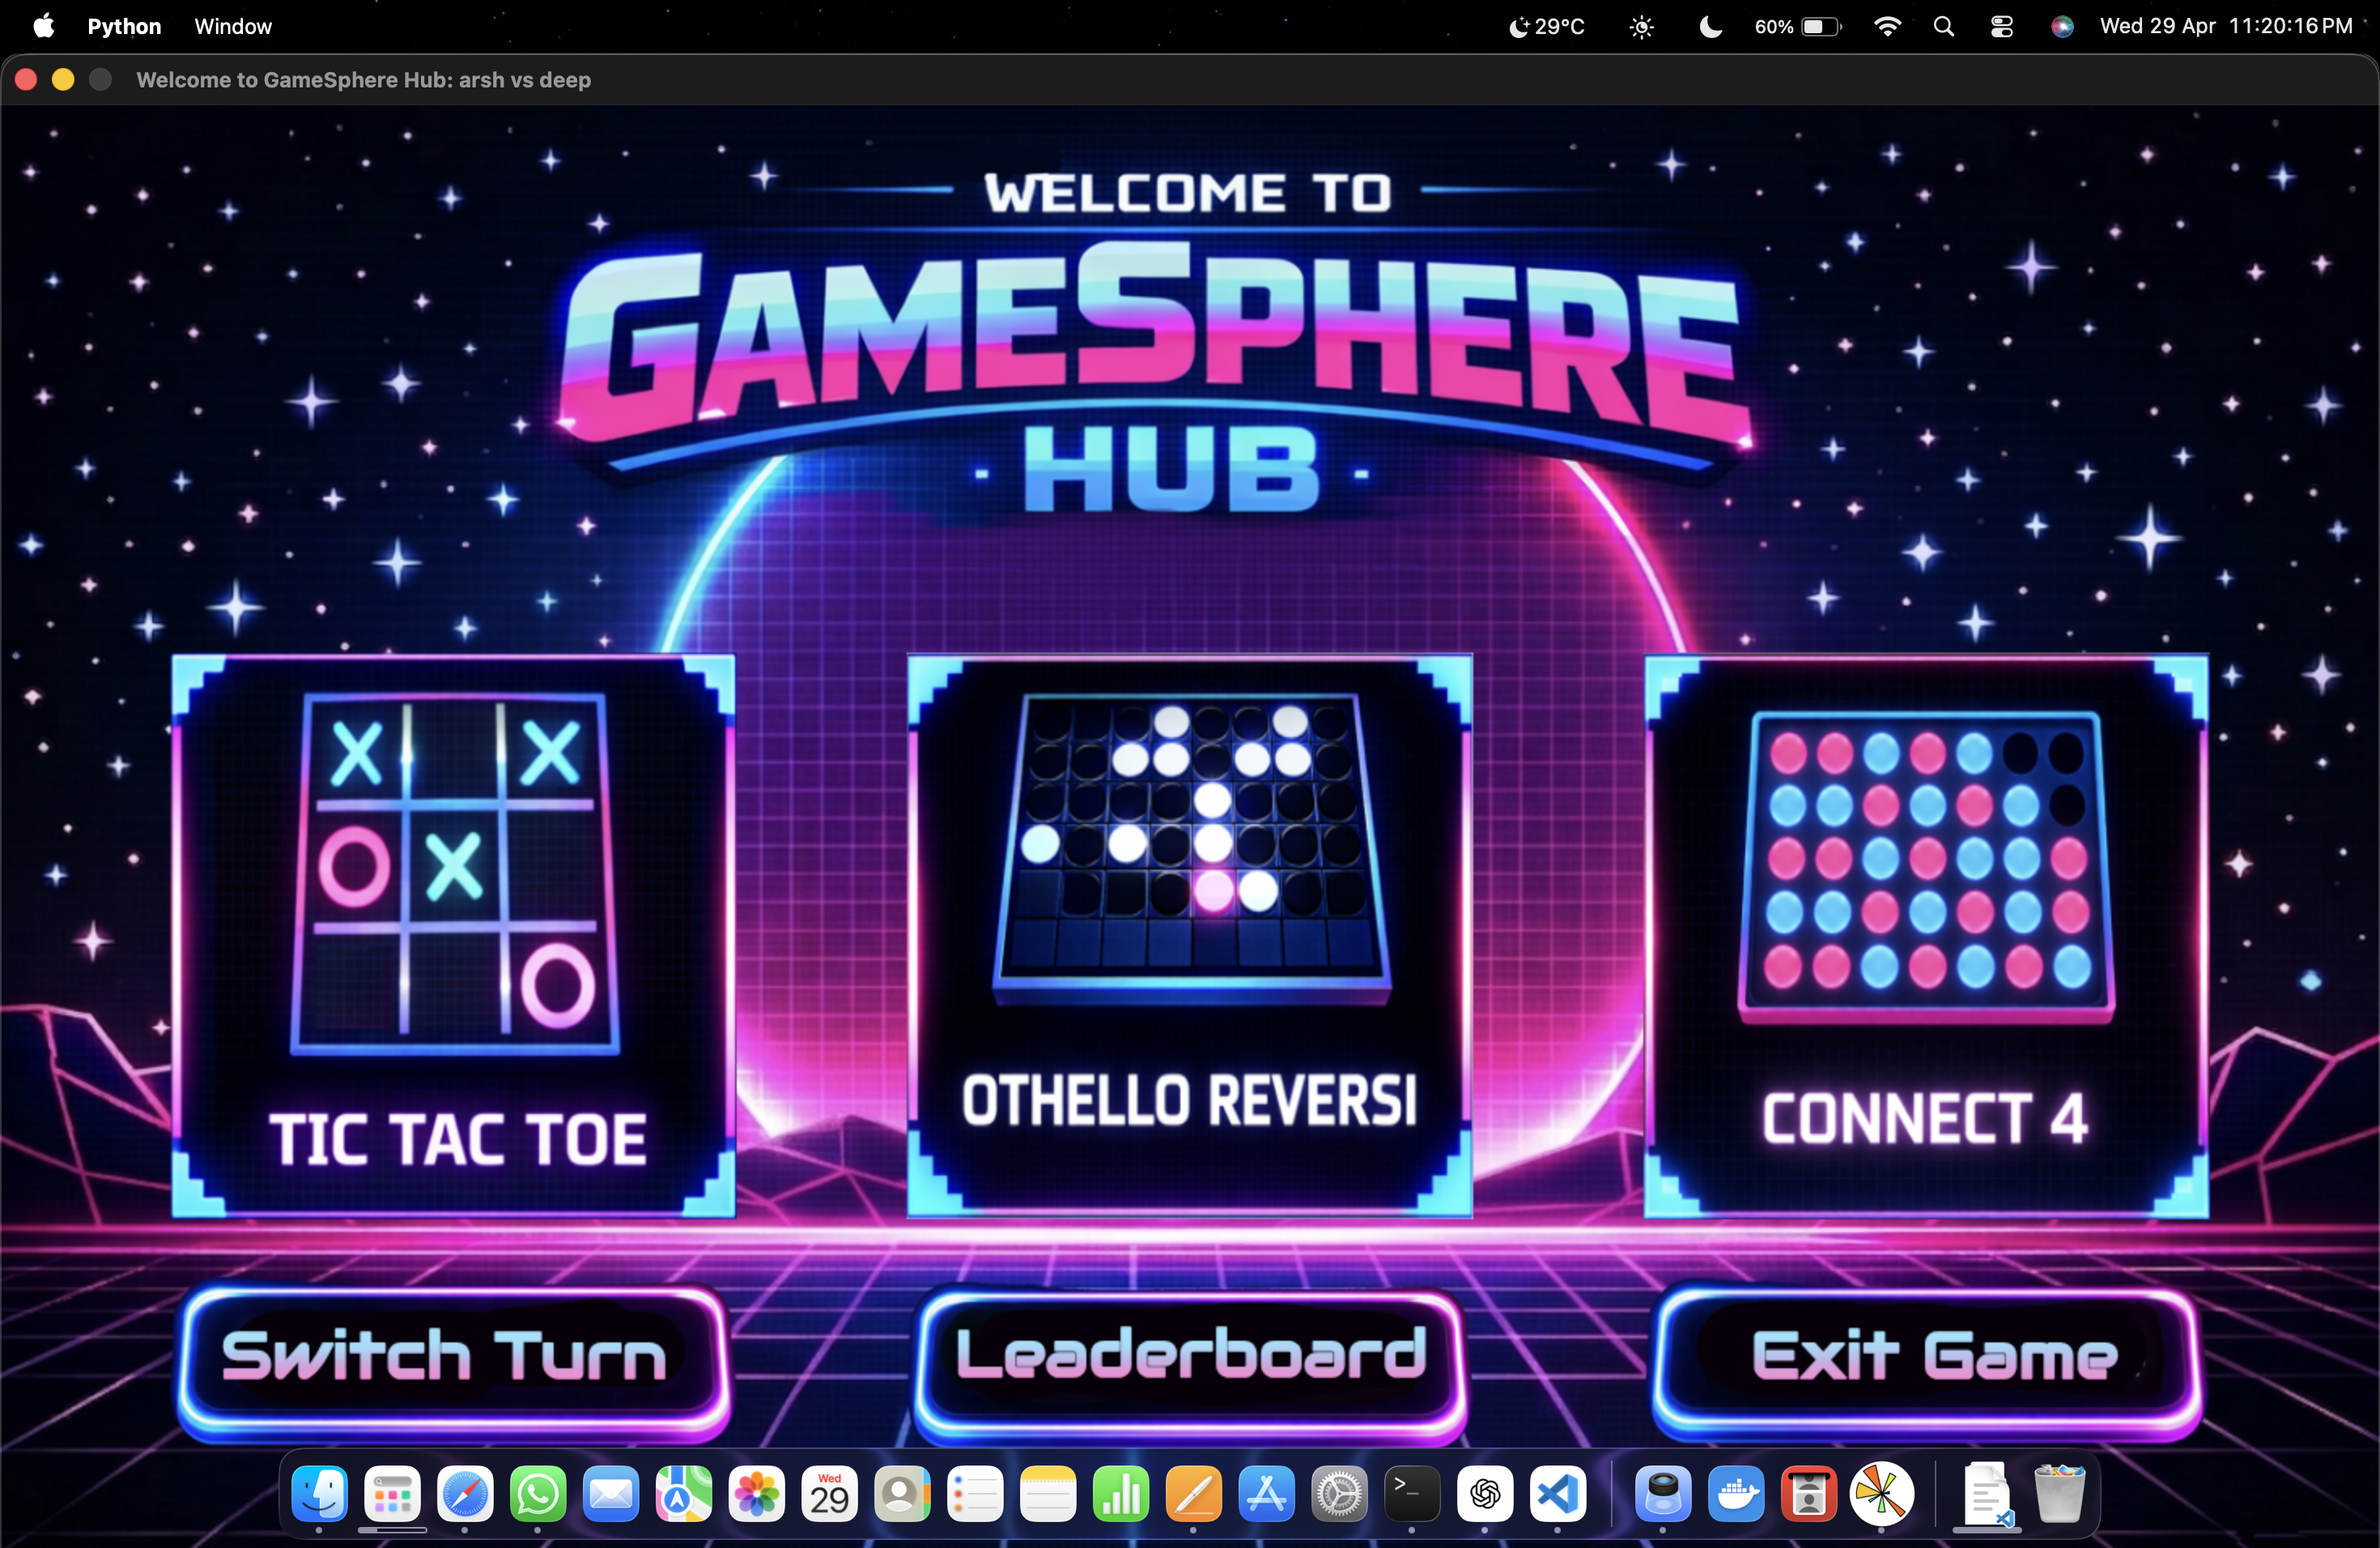
\includegraphics[width=\linewidth]{s1.png}
        \caption{Main Menu}
    \end{minipage}
    \hfill
    \begin{minipage}[t]{0.49\textwidth}
        \centering
        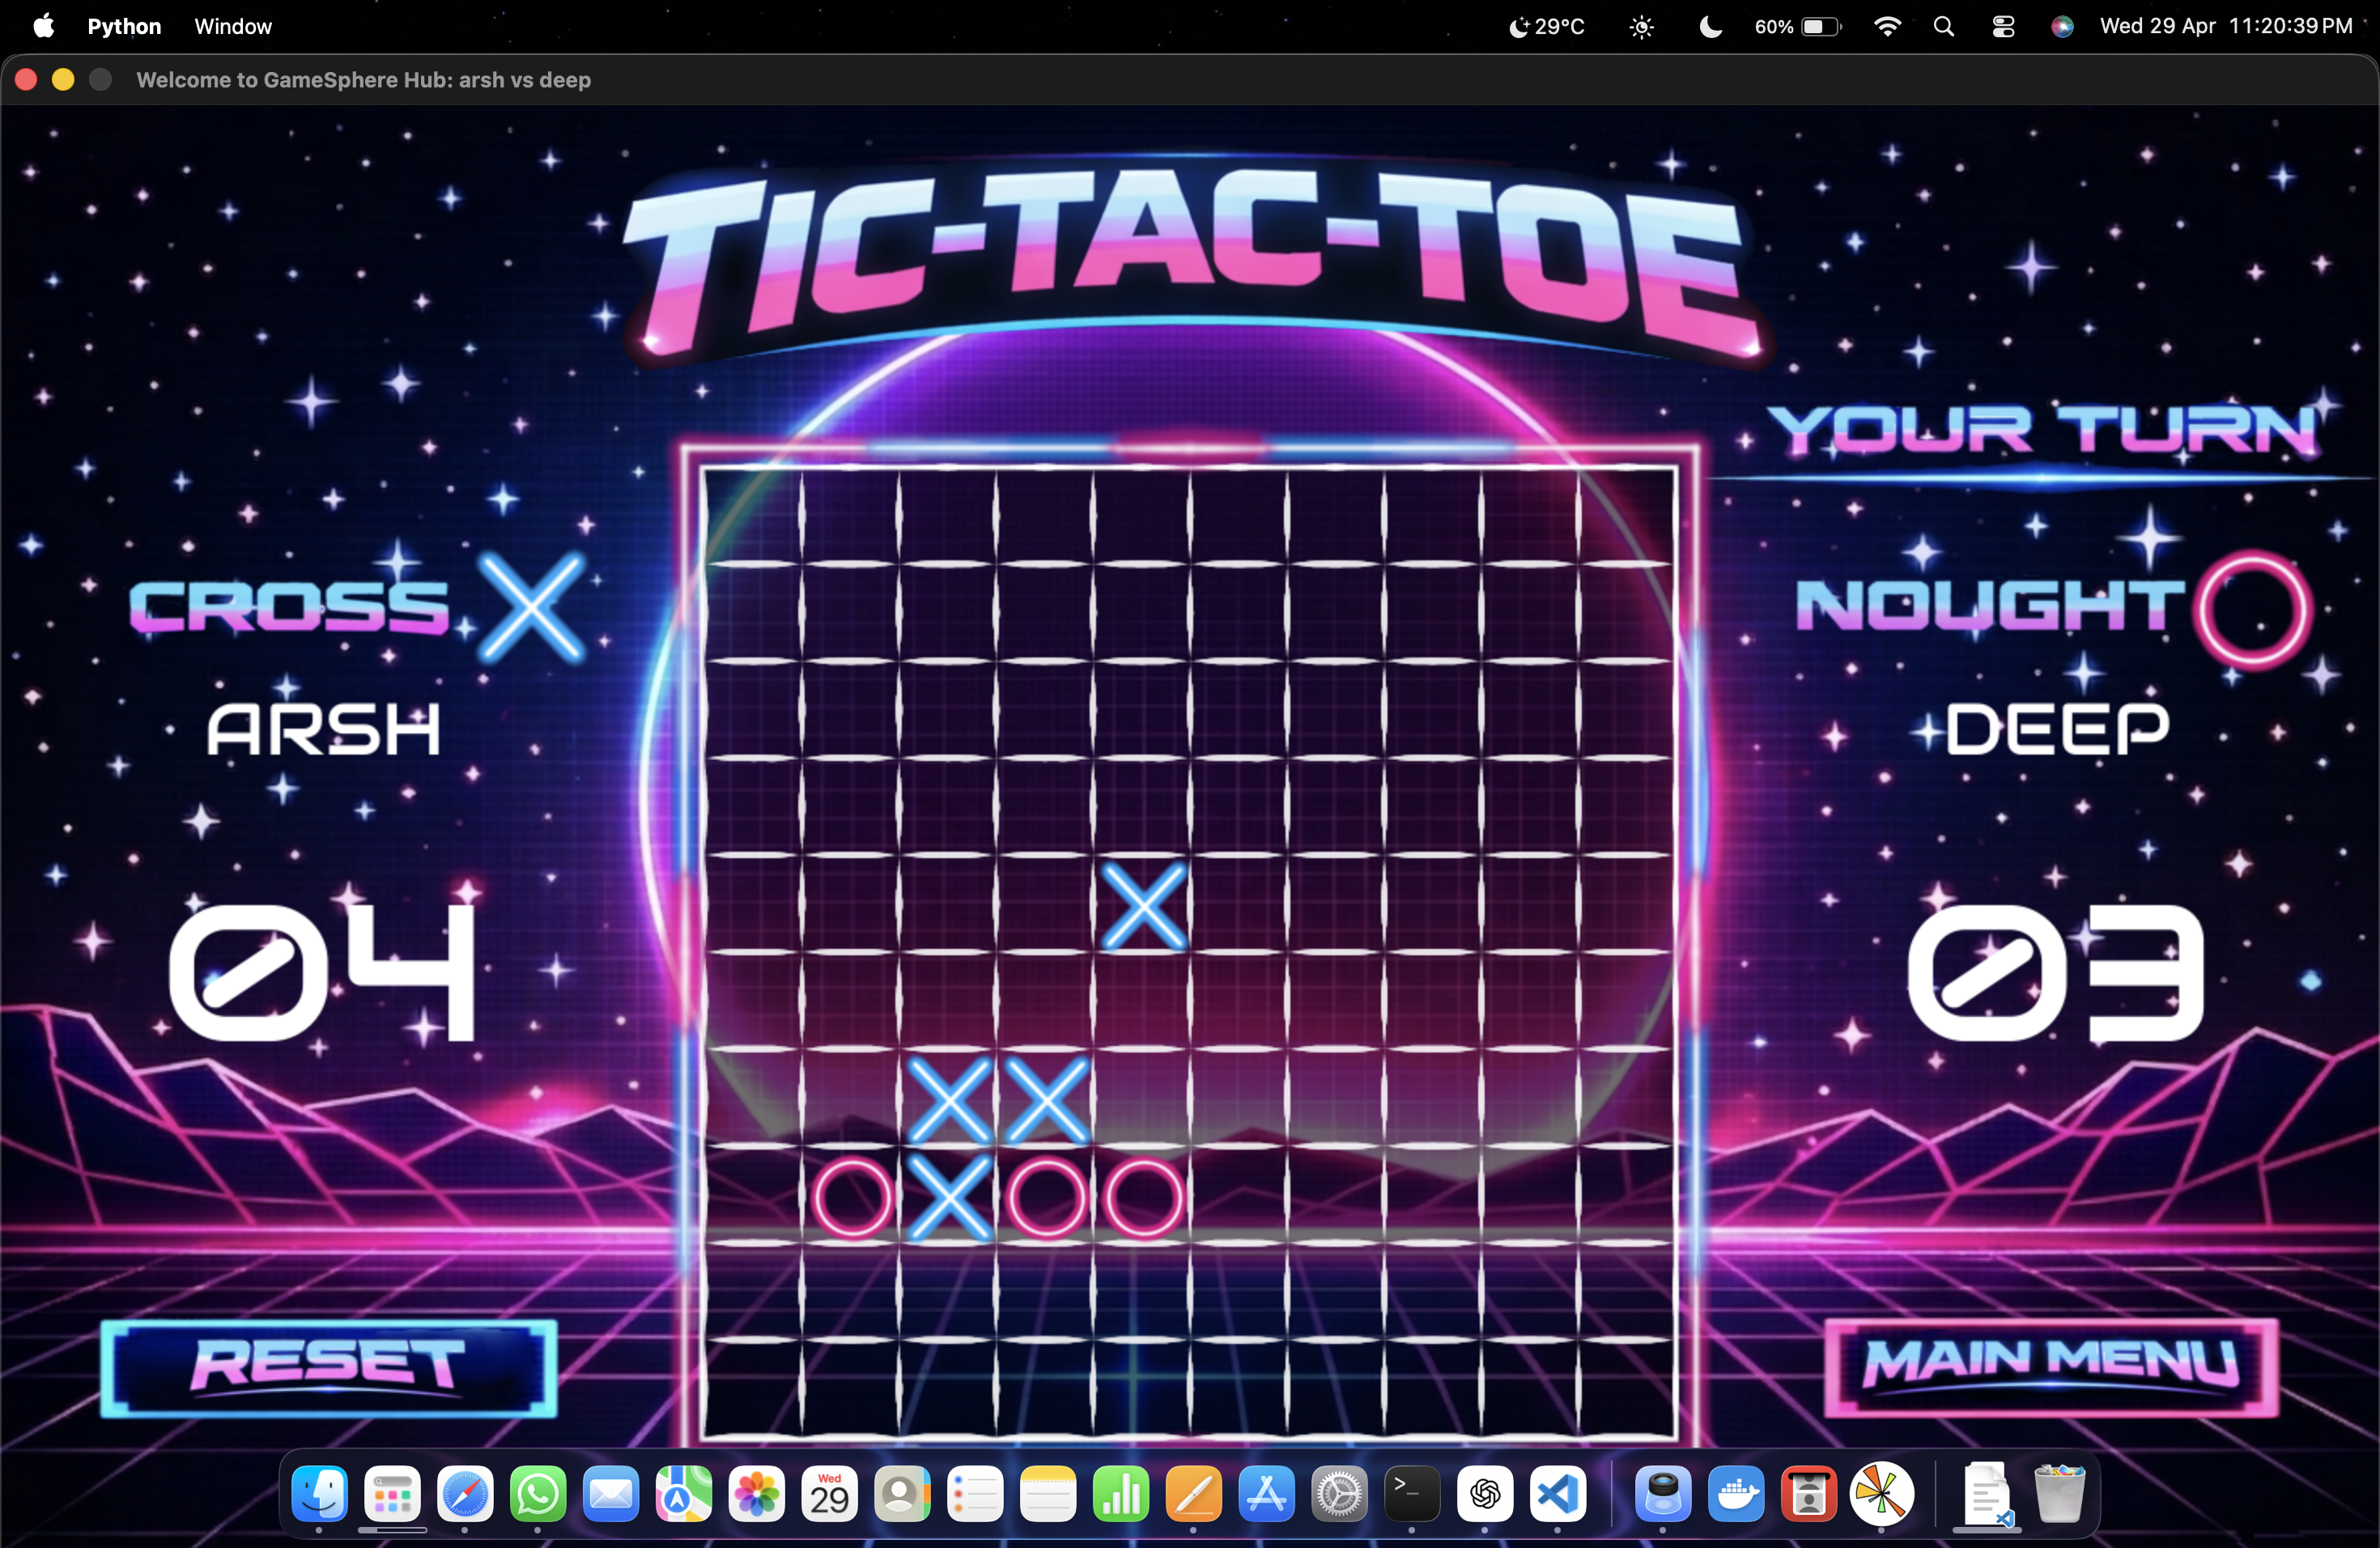
\includegraphics[width=\linewidth]{s2.png}
        \caption{TicTacToe Gameplay}
    \end{minipage}

\end{figure}

\clearpage

\begin{figure}[h]
    \centering

    \begin{minipage}[t]{0.49\textwidth}
        \centering
        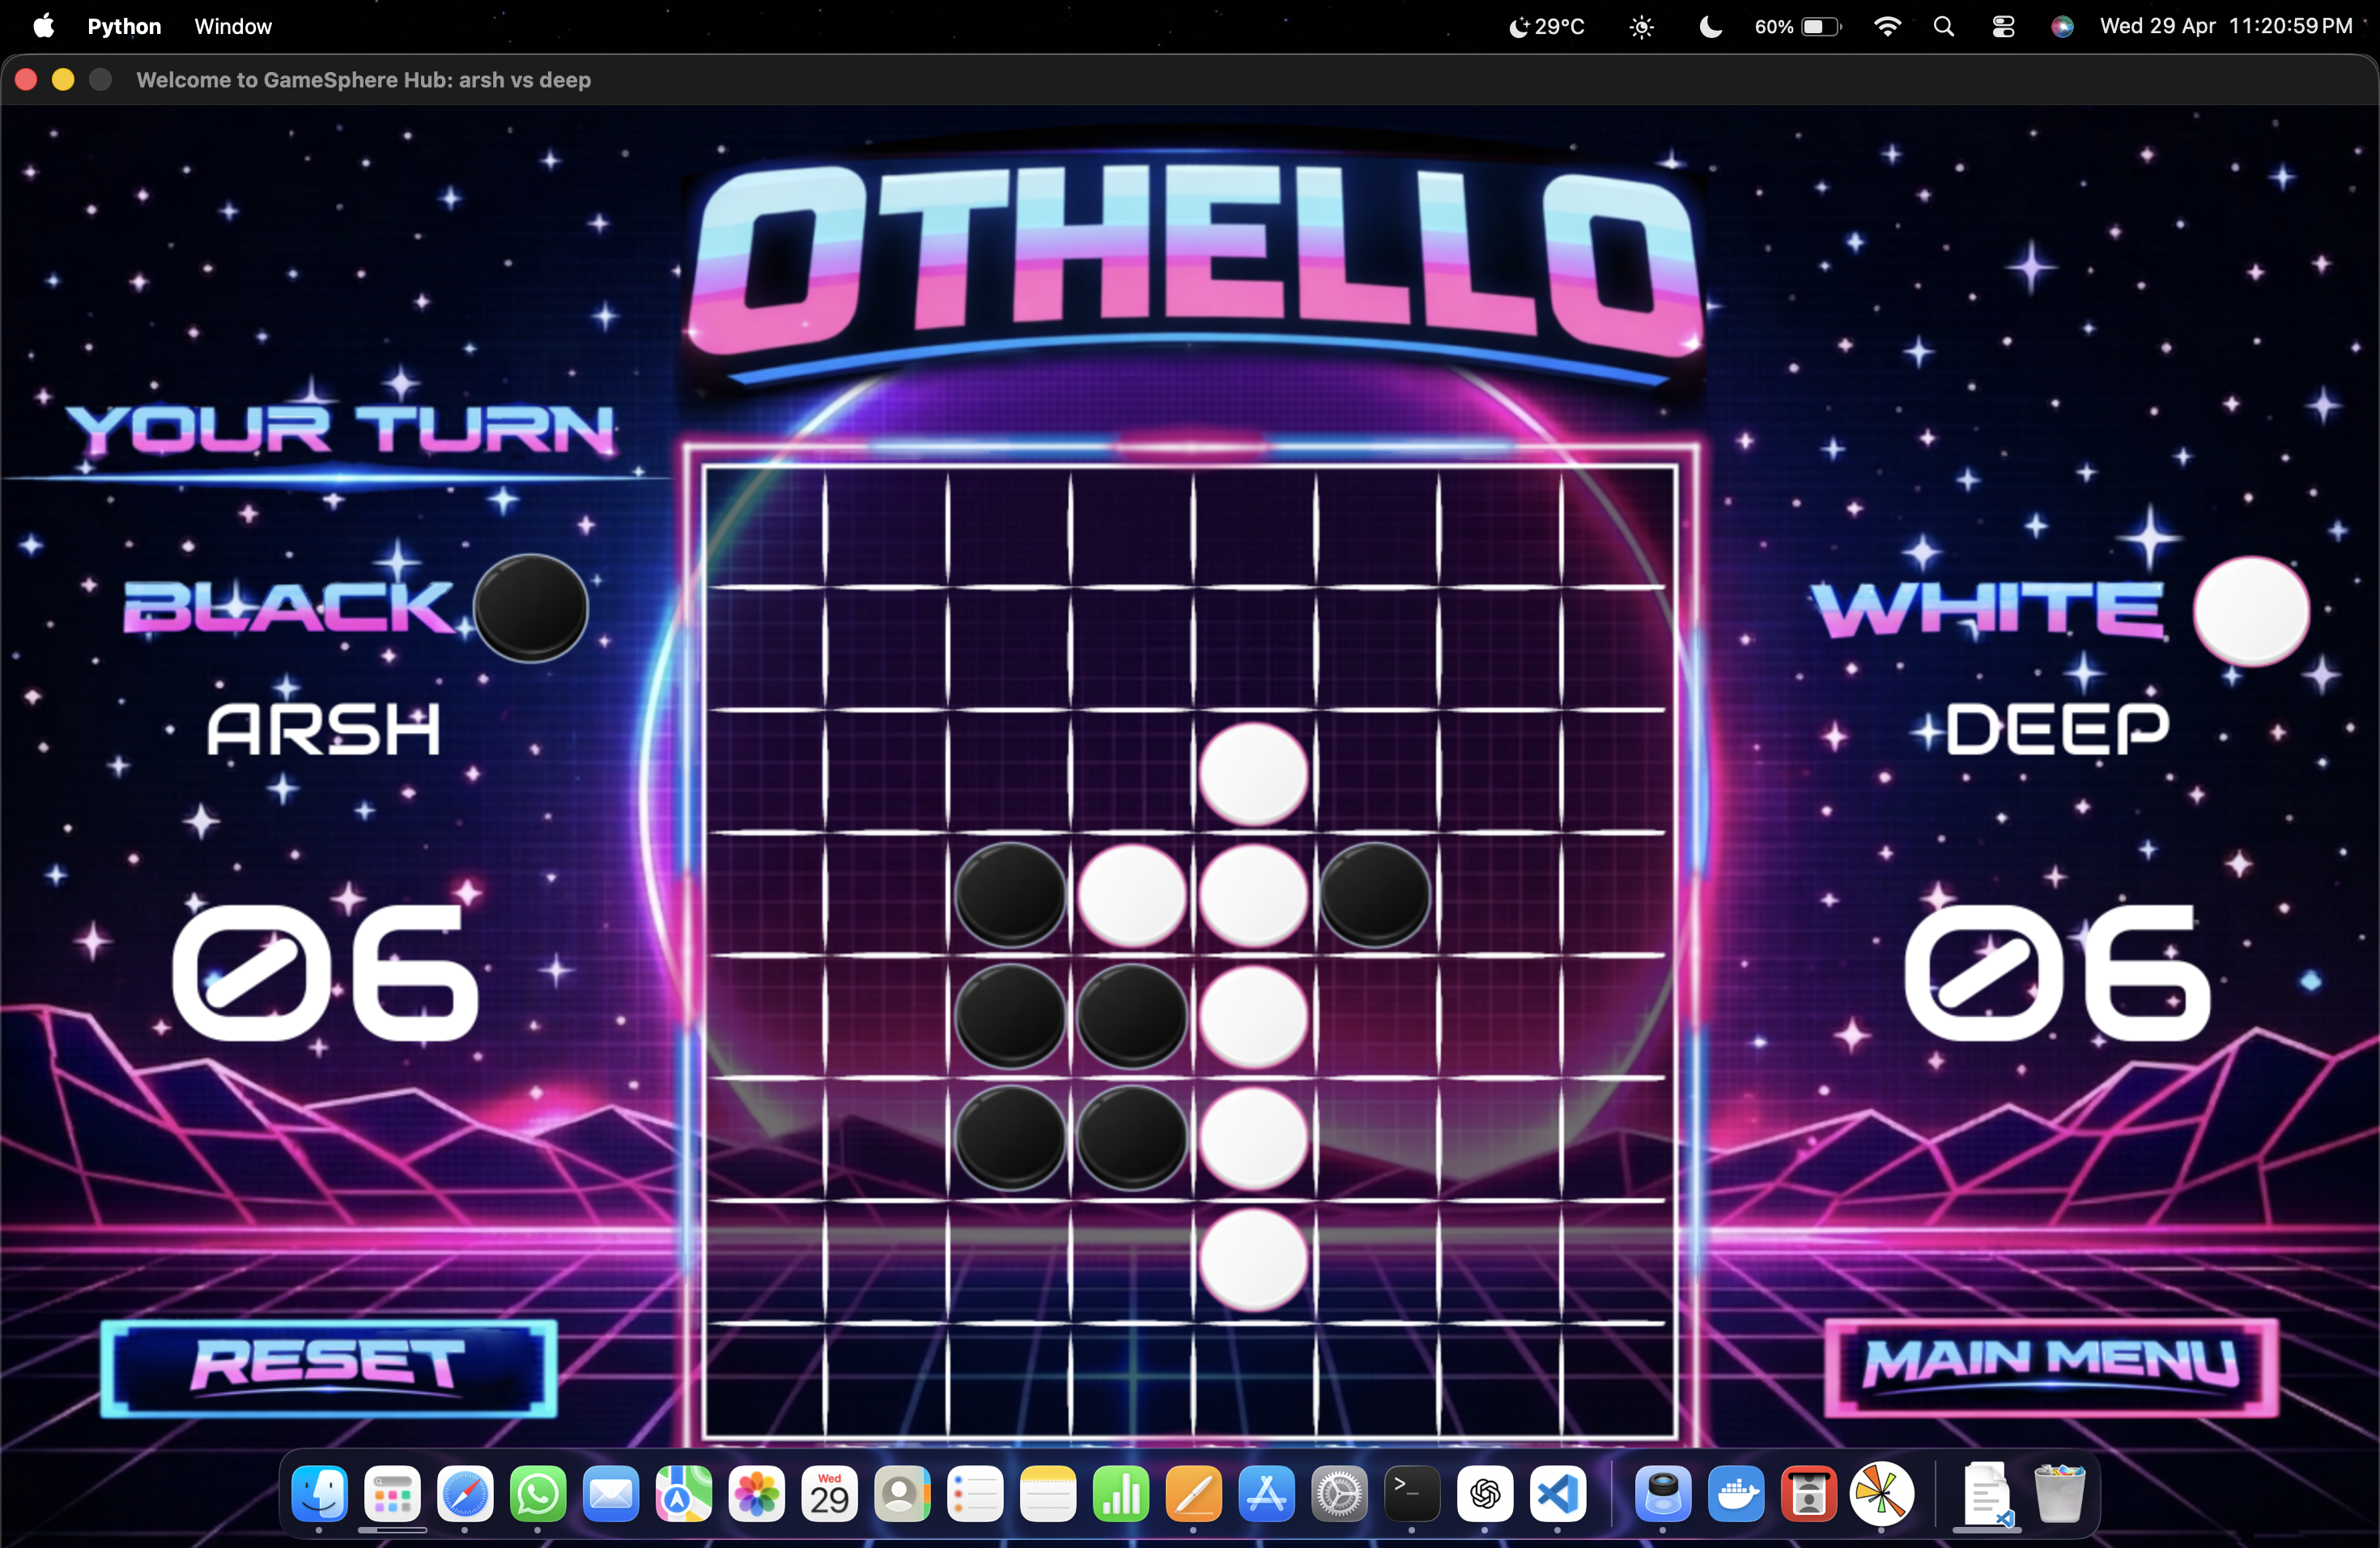
\includegraphics[width=\linewidth]{s3.png}
        \caption{Othello Gameplay}
    \end{minipage}
    \hfill
    \begin{minipage}[t]{0.49\textwidth}
        \centering
        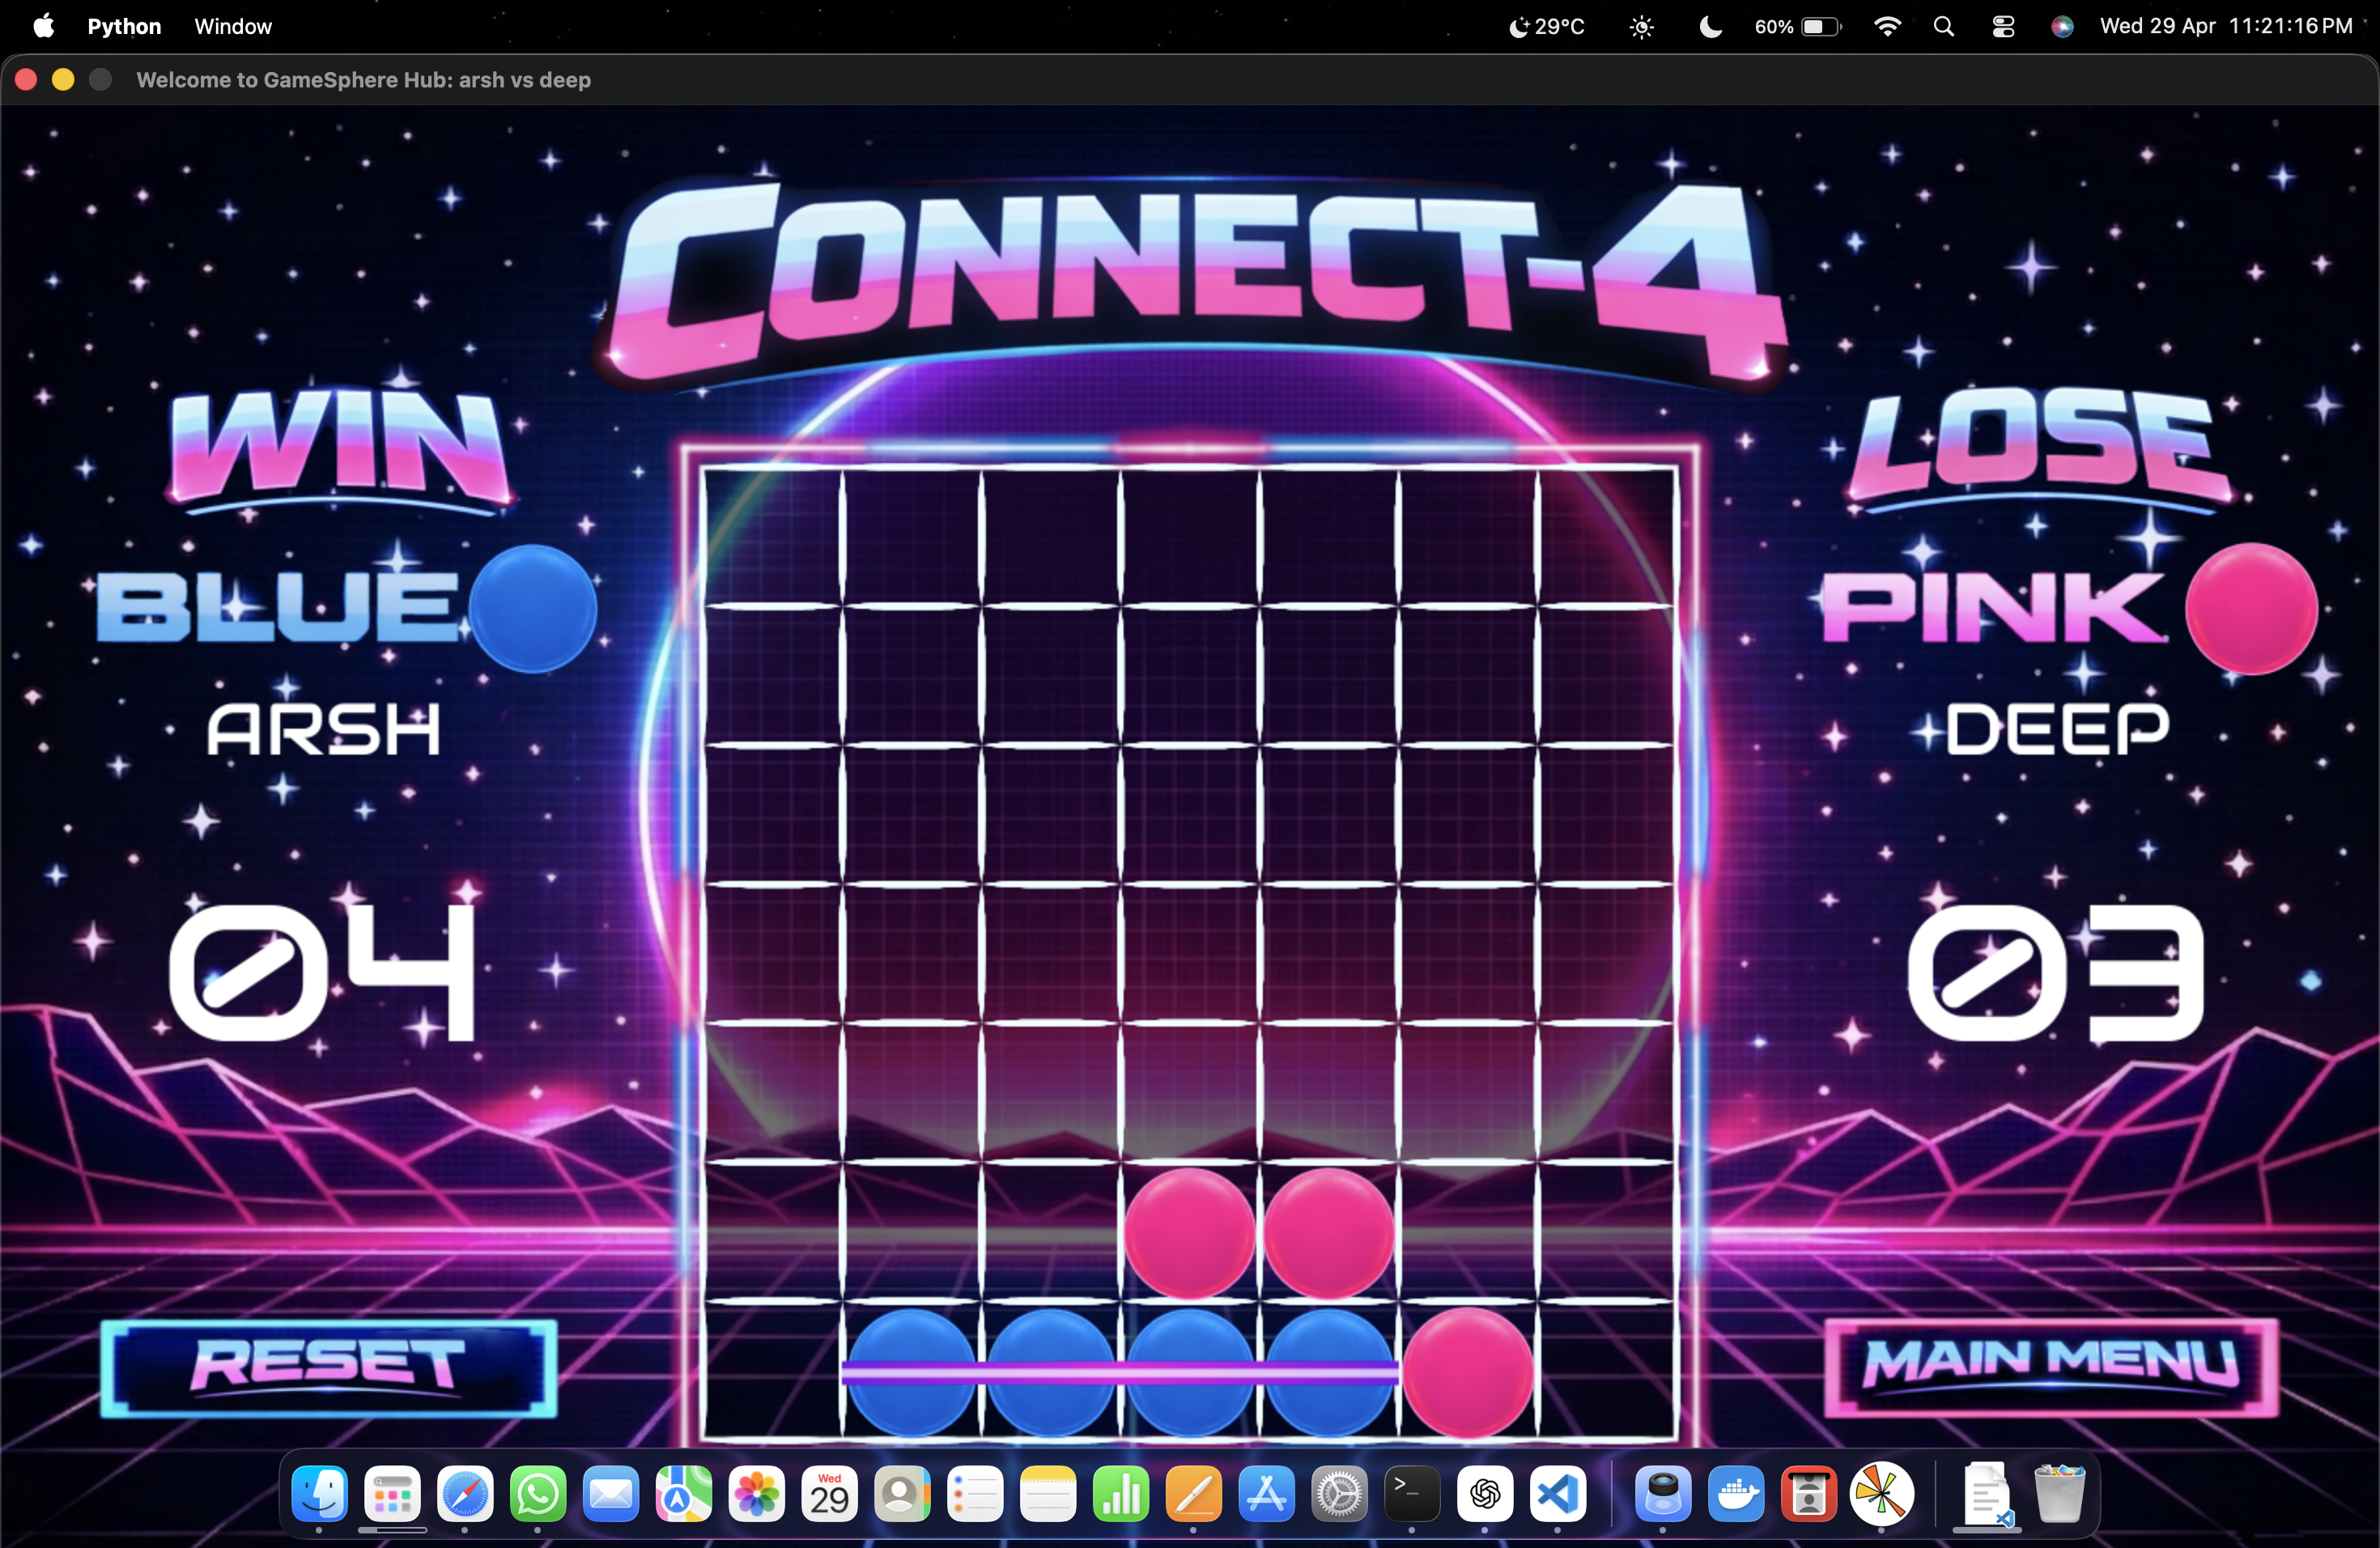
\includegraphics[width=\linewidth]{s4.png}
        \caption{Connect4 Gameplay}
    \end{minipage}

\end{figure}

\begin{figure}[h]
    \centering

    \begin{minipage}[t]{0.49\textwidth}
        \centering
        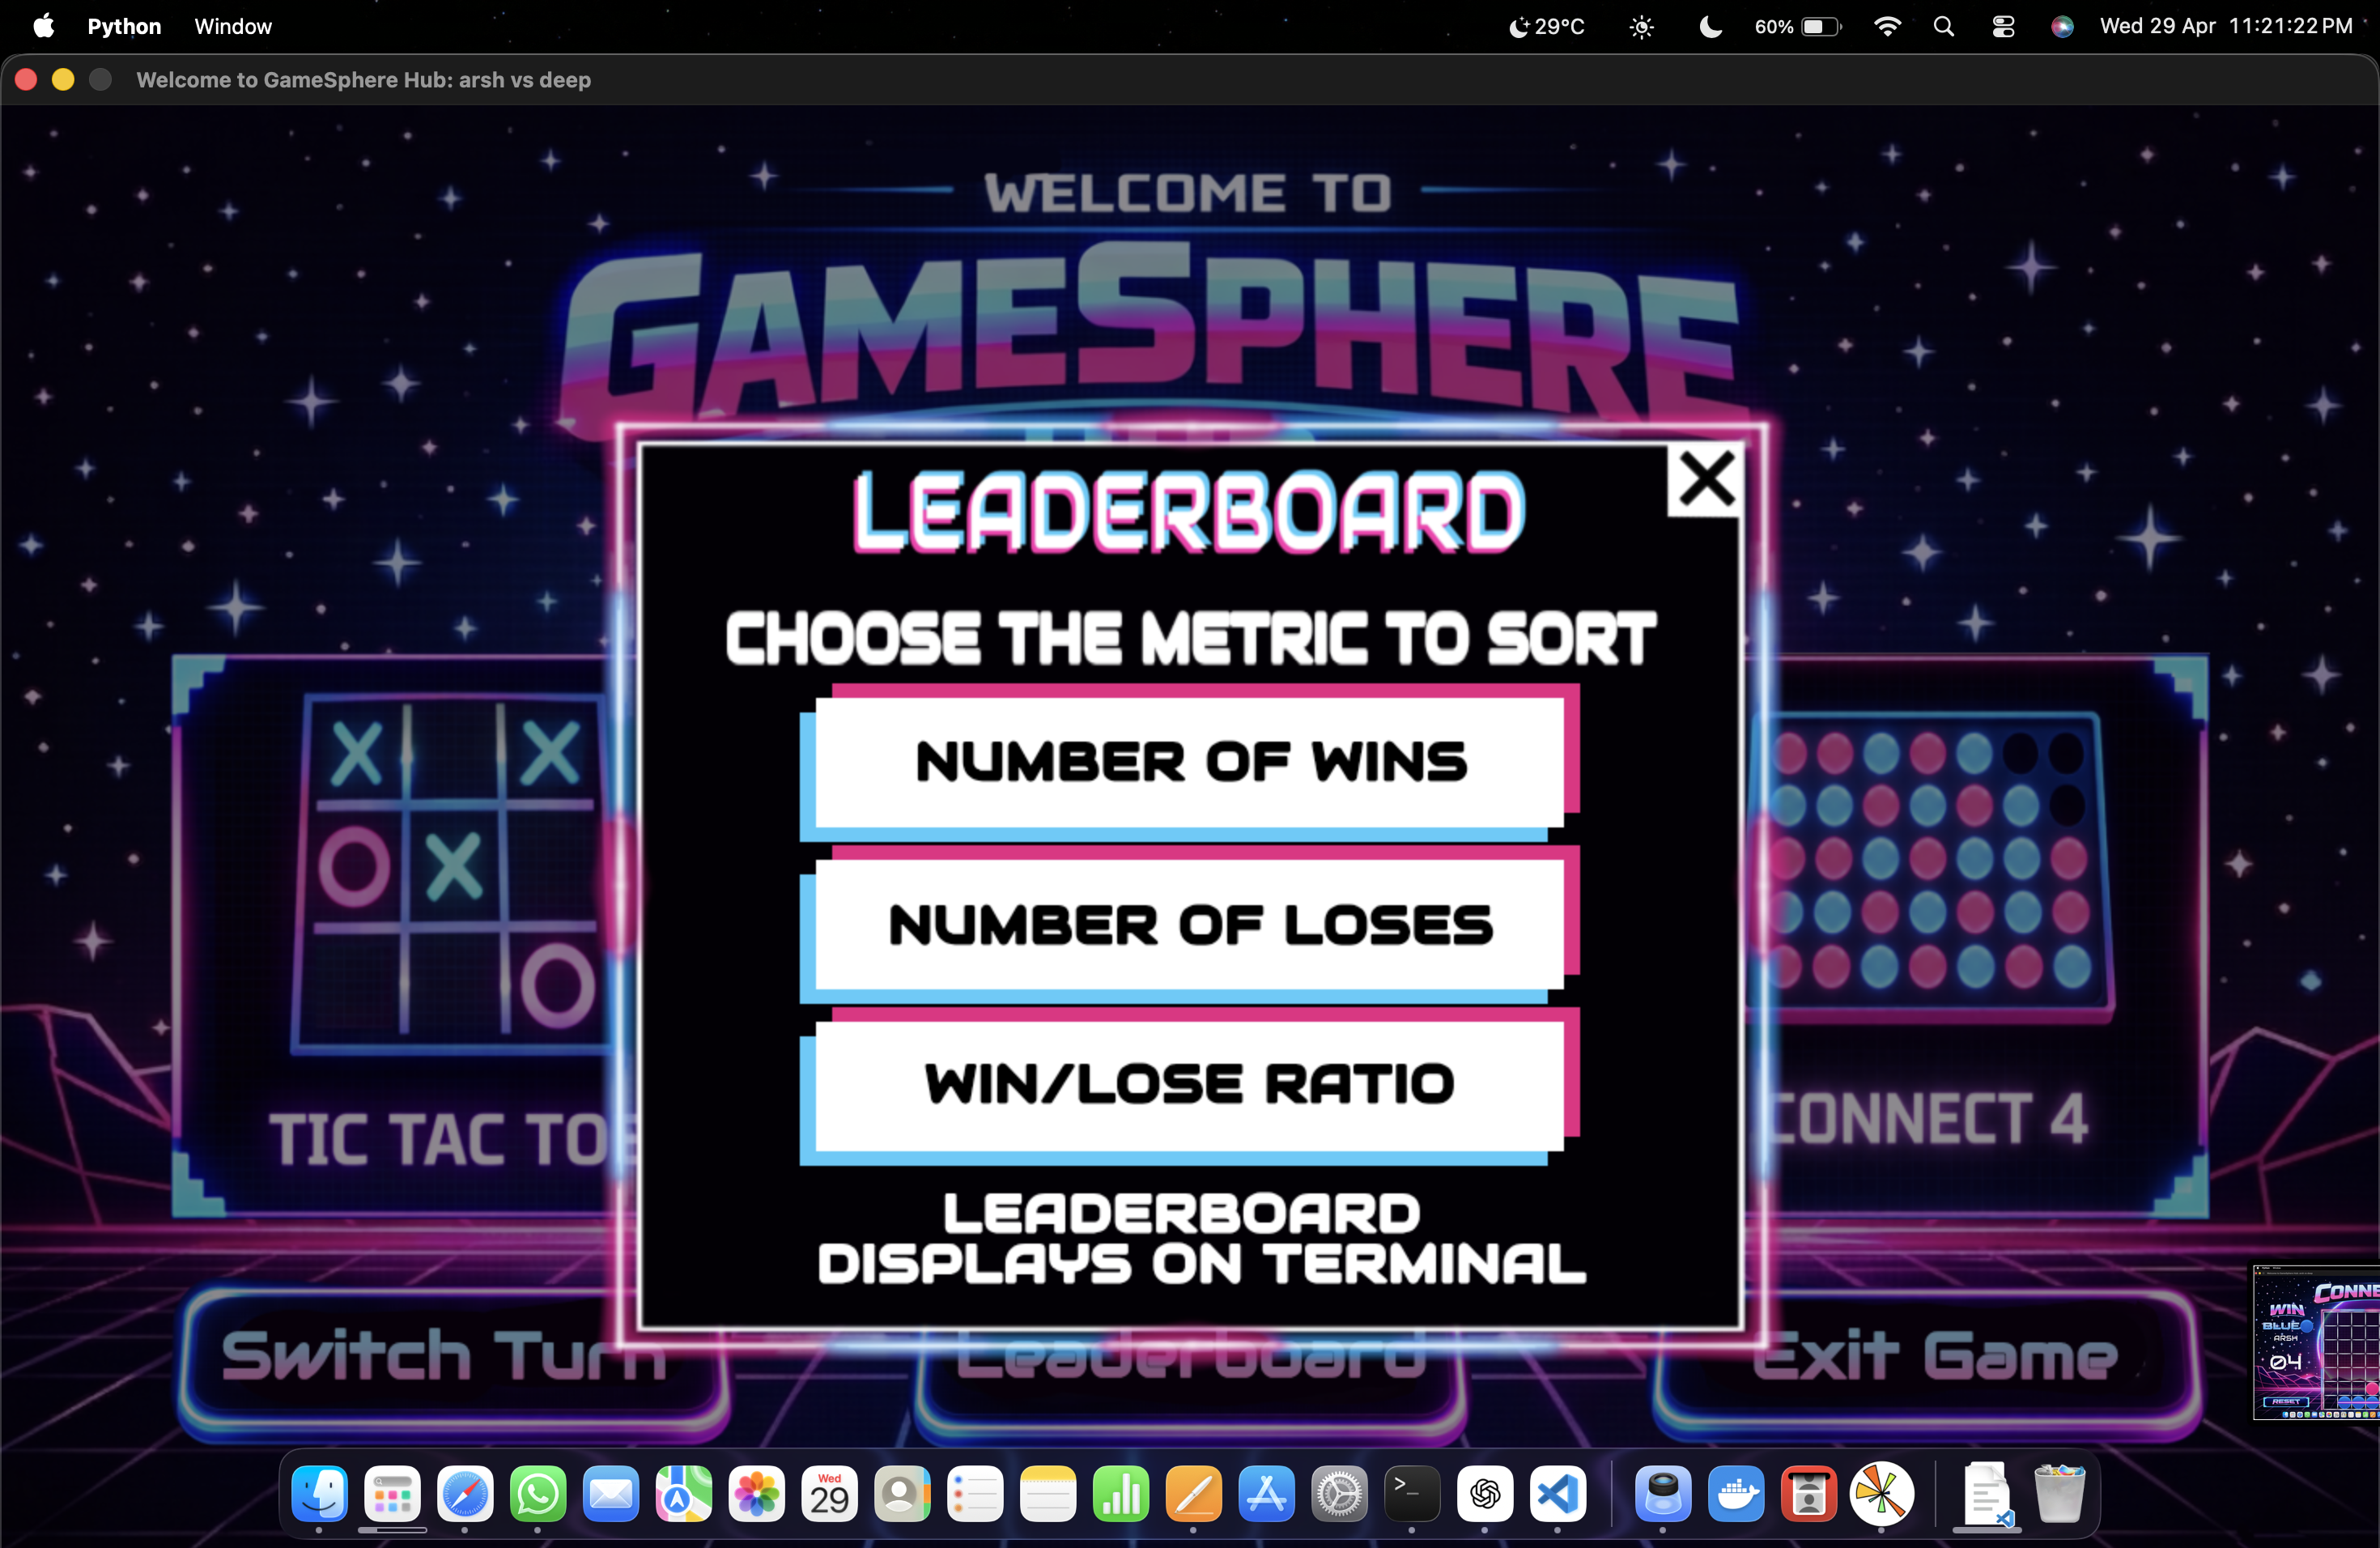
\includegraphics[width=\linewidth]{s5.png}
        \caption{Leaderboard Interface}
    \end{minipage}
    \hfill
    \begin{minipage}[t]{0.49\textwidth}
        \centering
        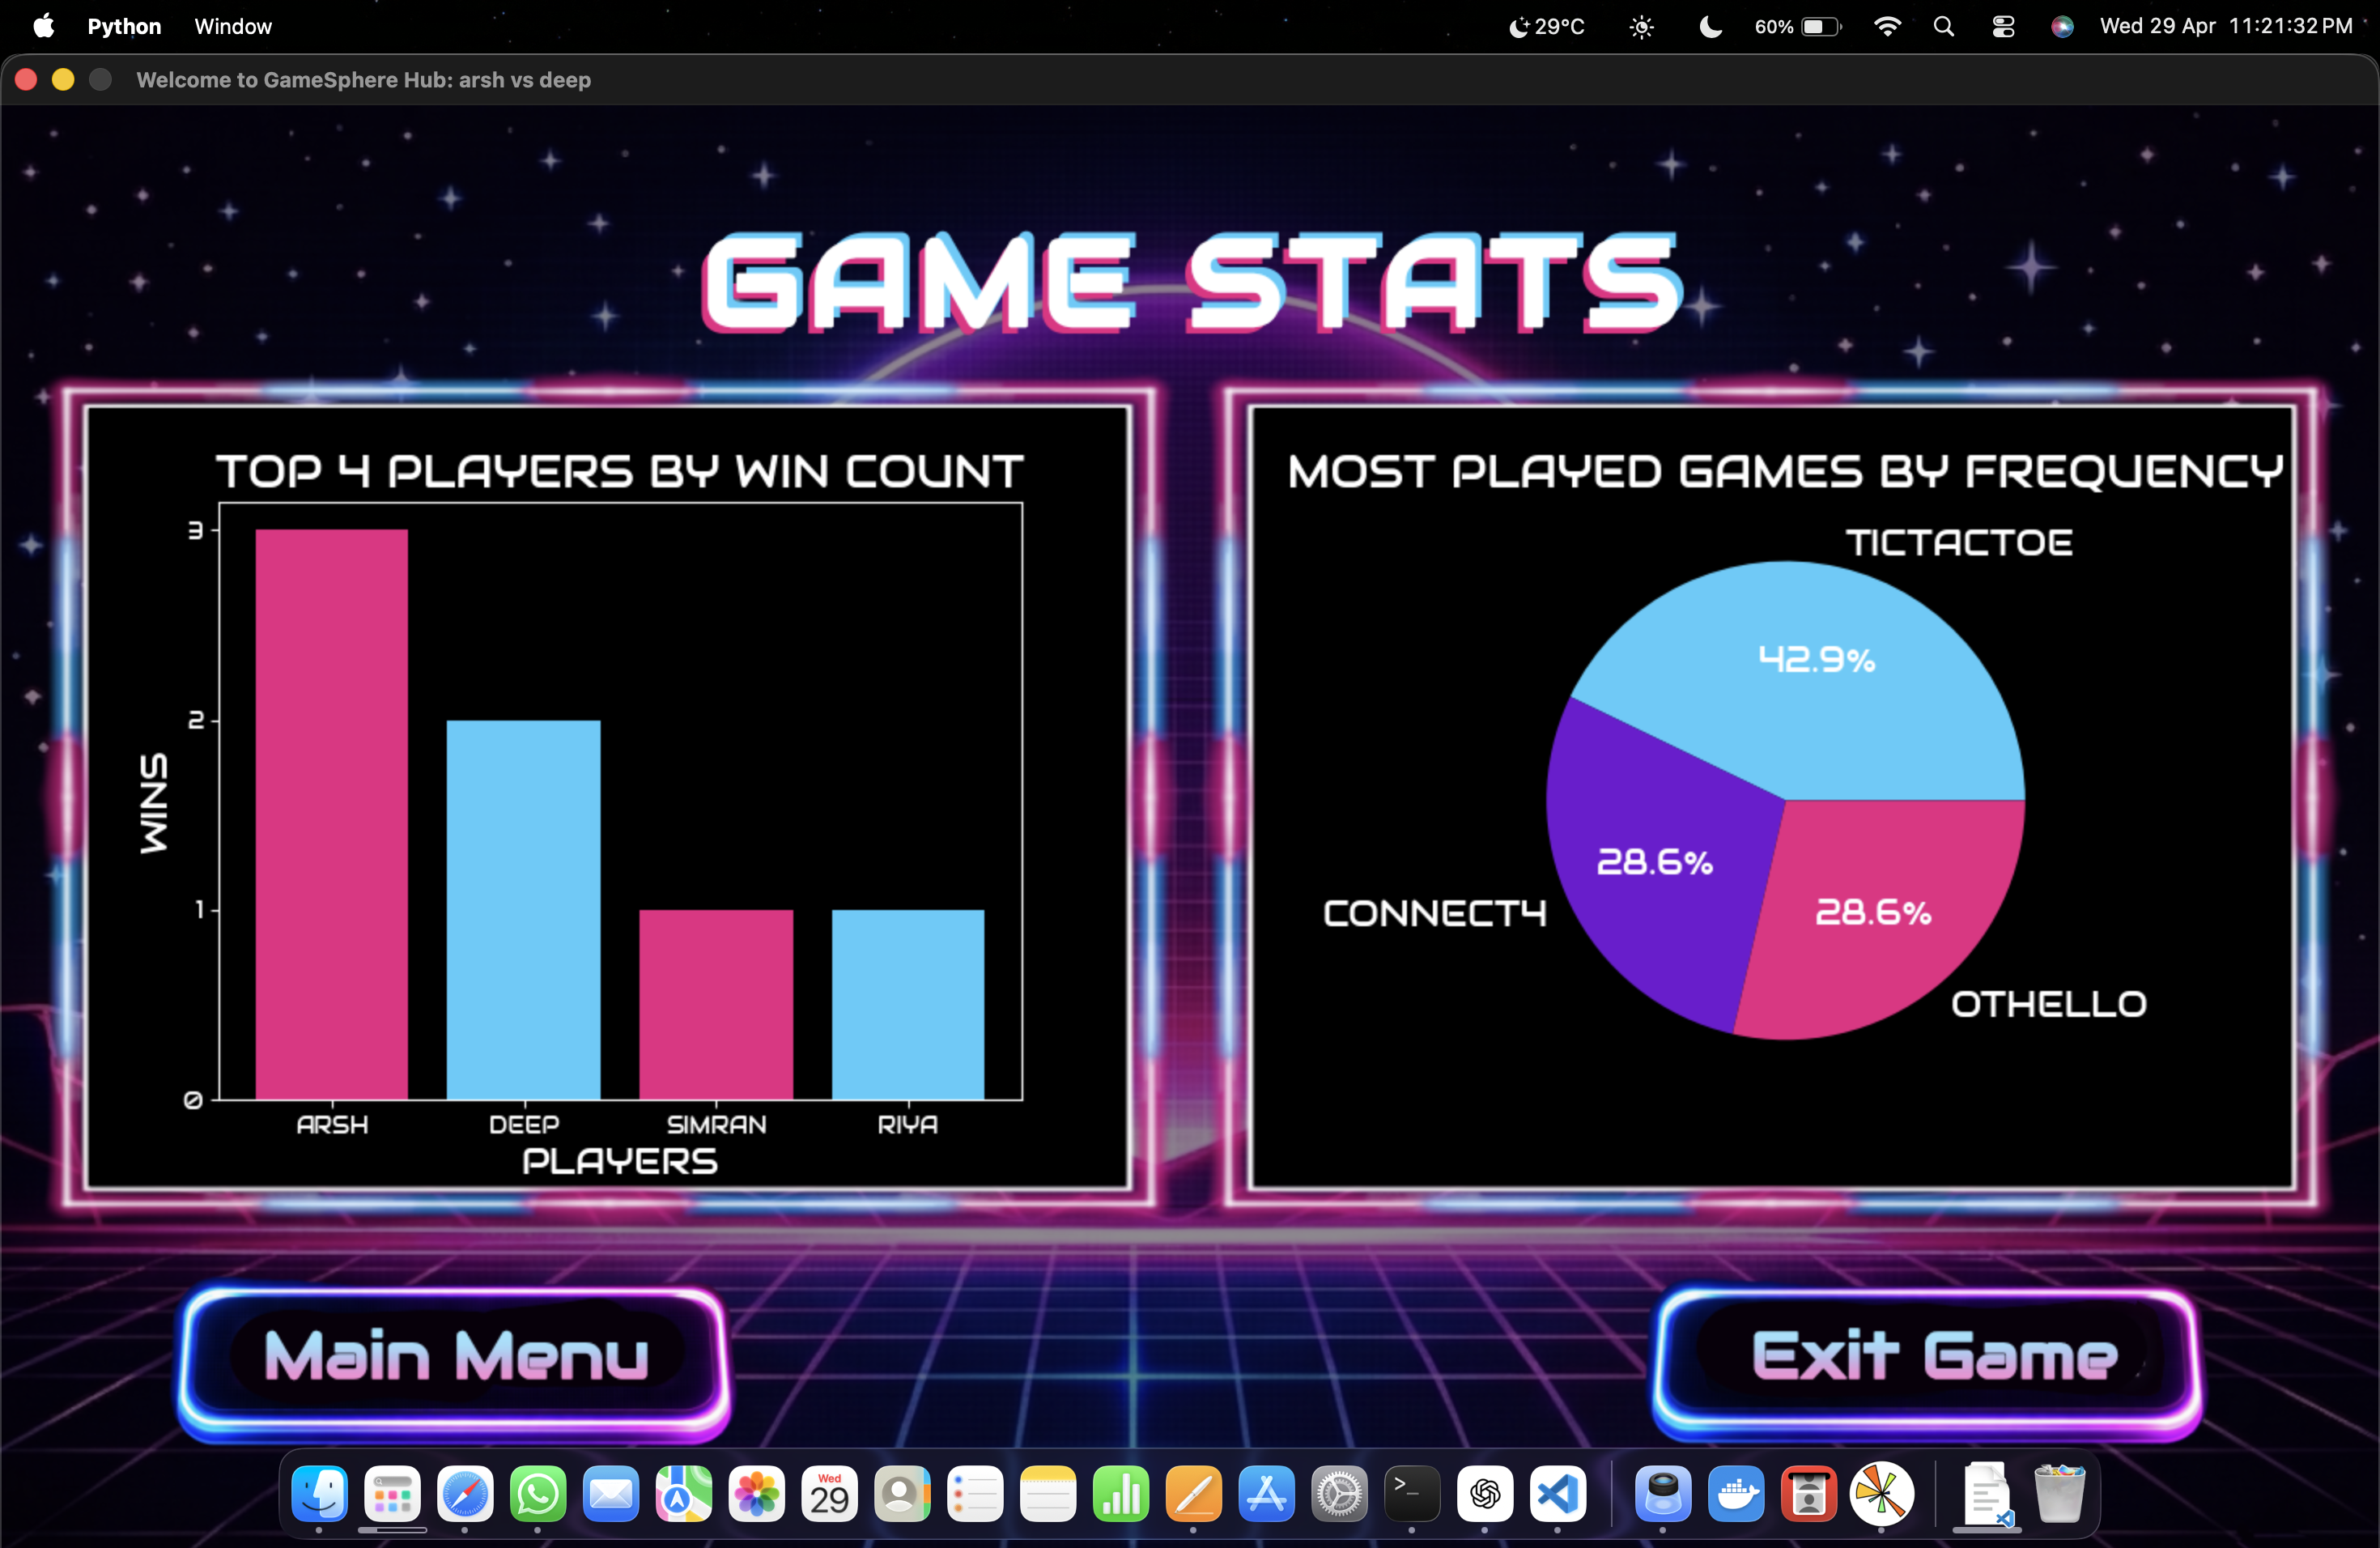
\includegraphics[width=\linewidth]{s6.png}
        \caption{Visualise Stats Interface}
    \end{minipage}

\end{figure}
%====================================================

\section{Retrospective}

\subsection{Major Challenges Faced}

\subsubsection{Othello Move Validation}

Othello required complex checking in all eight directions for valid moves and disc flipping.

\textbf{Solution:} Used systematic directional traversal and stored valid moves in a set for efficient checking.

\subsubsection{Win Detection Optimization in TicTacToe and Connect4}
Since loops were not allowed to be used in checking win condition, it required understanding of complex methods in numpy.
\textbf{Solution:} Used NumPy sliding window operations for optimized detection.

\subsubsection{Bash and Python Integration}

Passing data between Bash scripts and Python required careful handling.

\textbf{Solution:} Used command-line arguments and subprocess execution.

\subsubsection{UI Asset Management}

Managing images, fonts, and scaling required repeated adjustments.

\textbf{Solution:} Standardized asset loading using the base Game class.

\subsection{Future Improvements}

\begin{itemize}
    \item AI single-player mode
    \item Better animations and sound effects
    \item Tournament mode
    \item Achievement and ranking system
    \item Adding more board game like Checkers, Ludo, Snake \& Ladders
\end{itemize}

%====================================================

\section{References}

\begin{itemize}
    \item Pygame Documentation: \url{https://www.pygame.org/docs/}
    \item NumPy Documentation: \url{https://numpy.org/doc/}
    \item Matplotlib Documentation: \url{https://matplotlib.org/}
    \item Python Official Docs: \url{https://docs.python.org/3/}
\end{itemize}

\end{document}